\section{Fault Injection using Emulation and Simulation Tools}

While Software-Implemented Fault Injection is effective for assessing software resilience, it is often limited by its inability to access low-level hardware states (such as pipeline registers) or accurately model timing-dependent hardware behaviors. Conversely, physical hardware injection offers ultimate realism but lacks observability and is often prohibitively expensive. Emulation and simulation-based fault injection serve as a crucial middle ground, bridging this gap by utilizing models to inject hardware-level faults while maintaining the high controllability and visibility typical of software approaches.

\subsection{Simulation vs. Emulation}
Simulation-based injection typically uses Instruction Set Architecture (ISA) simulators or Register Transfer Level (RTL) models. It offers high controllability and visibility, allowing injection into any architectural state (e.g., hidden pipeline registers). However, it often trades execution speed for accuracy and is bound by the model limitations, where it cannot simulate certain hardware features such as timers and exceptions.

On the other hand, emulation-based injection is highly accurate as it is able to record the real behavior of the device.
However, while gaining in accuracy it lacks in speed and as a result emulation campaigns often last hours. Moreover, this performance comes at the cost of visibility; unlike simulation, emulation is limited to the resources exposed by the hardware interface, often leaving internal micro-architectural structures (such as pipeline registers) inaccessible for injection or monitoring.

\subsection{Case Study: Evaluation of fault injection tools for reliability estimation of microprocessor-based embedded systems}
A study by Aponte-Moreno et al. \cite{EmulationSite} presents a rigorous quantitative comparison between simulation and emulation tools. The researchers evaluated the reliability of a Texas Instruments MSP430 microcontroller using three distinct tools:
\begin{itemize}
    \item \textbf{MiFIT:} A modular, open-source ISA simulator.
    \item \textbf{Naken-FIM:} A modified instruction-accurate simulator with enhanced trace capabilities.
    \item \textbf{FIM:} An emulation-based framework utilizing the On-Chip Debugging (OCD) infrastructure of the physical MSP430 device.
\end{itemize}

The study injected bit-flips into the register file and memory sections (.data, .stack, .text) while running standard benchmarks (Euler, QuickSort, Matrix Multiplication) per clock cycle or per instruction, in the case of simulators (Figure \ref{fig:Percentage}). The results were compared against ground-truth data from neutron beam irradiation experiments at the Los Alamos Neutron Science Center (LANSCE).

\begin{figure}[htbp]
    \centering
    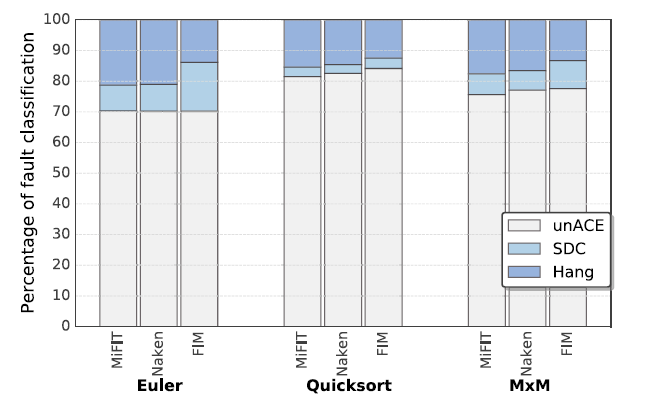
\includegraphics[width=0.9\linewidth]{assets/Percentage of fault classification.png}
    \caption{Percentage of fault classification for each benchmark.}
    \label{fig:Percentage}
\end{figure}

The comparison revealed that while simulation tools are faster, they can overestimate certain failure modes.

At first, the simulation tools (MiFIT and Naken) showed consistent results with each other, with differences in fault classification (e.g., Silent Data Corruption vs. Hang) of less than 3.3\% for the register file. However, they were significantly off from the emulation tool's results, and gave a reliability estimate that was 10\% lower.

More specifically, significant deviations were observed in critical registers such as the Program Counter (R0), the Stack Pointer (R1) and other non-critical registers depending on the benchmark application (Figure \ref{fig:Registers}). These differences were mainly due to the limitations of the simulator models; For example, in the Euler benchmark, faults in register R6 caused a "Hang" in the simulator but a "Silent Data Corruption" (SDC) in the emulator. This difference was attributed to the simulators' simplified handling of execution time. The researchers observed that the real hardware continued executing "trash code" longer than the simulator allowed, thus, misclassifying the fault for only a few cycles of discrepancy. Extending the simulator's timeout limit significantly reduced this gap.

\begin{figure}[htbp]
    \centering
    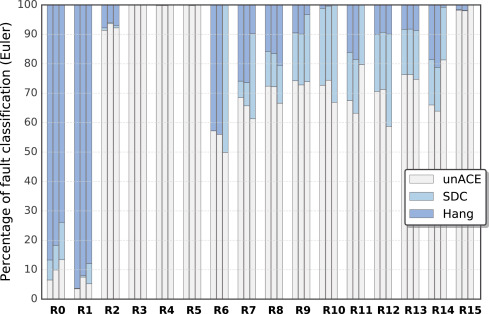
\includegraphics[width=0.9\linewidth]{assets/register-faults.jpg}
    \caption{Percentages of fault classification in the register file by fault injection tool (MiFIT, Naken, and FIM) for Euler}
    \label{fig:Registers}
\end{figure}

Furthermore, simulation tools often lacked accurate models for hardware exceptions. Faults injected into the stack pointer (SP) on the real device often triggered system resets or traps, that the ISA simulators processed as valid jumps to uninitialized memory. This also led to divergent failure classifications.

Overall, the study concludes that ISA-level simulation is highly effective for preliminary design space exploration, offering a speed advantage for tuning fault mitigation techniques. However, for final validation, emulation or hybrid approaches are necessary to capture micro-architectural behaviors (such as pipeline stalls and hardware exceptions) that simulators often abstract away.

\subsection{Case Study: RTL-Based Reliability and Resource Analysis of Spaceborne FPGAs}
While ISA-level simulation focuses on software behavior, simulation at the Register Transfer Level (RTL) enables the evaluation of hardware fault tolerance mechanisms (FTMs) early in the design phase. A 2025 study by Kim et al. \cite{AerospaceSiteEmu} utilized this approach to analyze the trade-offs between reliability and resource utilization in spaceborne electronic systems.

The study targeted an AES-128 encryption circuit, a critical component for secure space communications. To assess reliability, the authors employed Statistical Fault Injection (SFI) using the \textit{Verilog Fault Injector} on the \textit{Icarus Verilog} simulator. They injected single-bit and multi-bit faults (reflecting Single Event Upsets) into the circuit's key expansion and round modules.

Unlike the software-focused metrics of ISA simulators, this RTL-based approach allowed for the calculation of the \textit{Architectural Vulnerability Factor} (AVF) alongside physical resource metrics defined as the Power-Delay-Area Product (PDAP):
\begin{equation}
    PDAP = Power \times Delay \times Area
\end{equation}
This metric provided a quantitative basis for comparing hardware redundancy (e.g., TMR) against information redundancy (e.g., Hamming Code)(Figure \ref{fig:Classification}).

\begin{figure} [htbp]
    \centering
    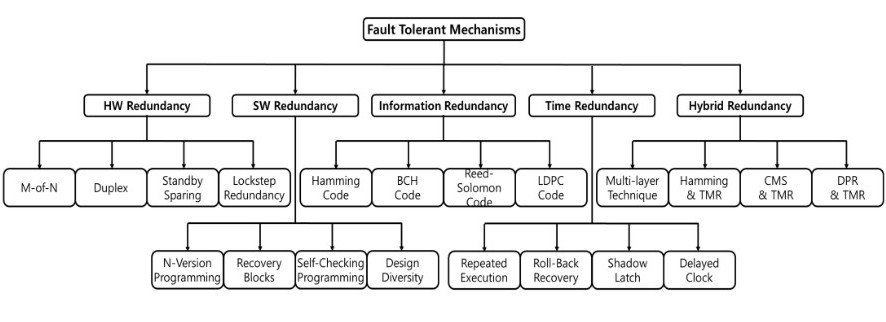
\includegraphics[width=0.9\linewidth] {assets/classification.jpg}
    \caption{Classification of fault-tolerant mechanisms for electronic equipment}
    \label{fig:Classification}
\end{figure}

The simulation results highlighted distinct trade-offs between the two redundancy categories:

\begin{itemize}
    \item \textbf{Information Redundancy:} The Hamming Code mechanism achieved high reliability, reducing the AVF significantly. However, it incurred a massive resource penalty, increasing the PDAP by approximately 355\% compared to the baseline due to the complexity of encoding/decoding logic.
    \item \textbf{Hardware Redundancy:} Triple Modular Redundancy (TMR) offered the most efficient balance. While its reliability was slightly lower than the most robust hybrid methods, it maintained a low resource overhead (PDAP), making it highly suitable for resource-constrained FPGA environments.
    \item \textbf{Hybrid Approaches:} A combined "Hamming \& TMR" mechanism yielded the highest reliability ($95.82\%$ fault masking) but at a prohibitive resource cost, with a PDAP increase of over 587\% (Figure \ref{fig:PDAP}).
\end{itemize}

\begin{figure} [htbp]
    \centering
    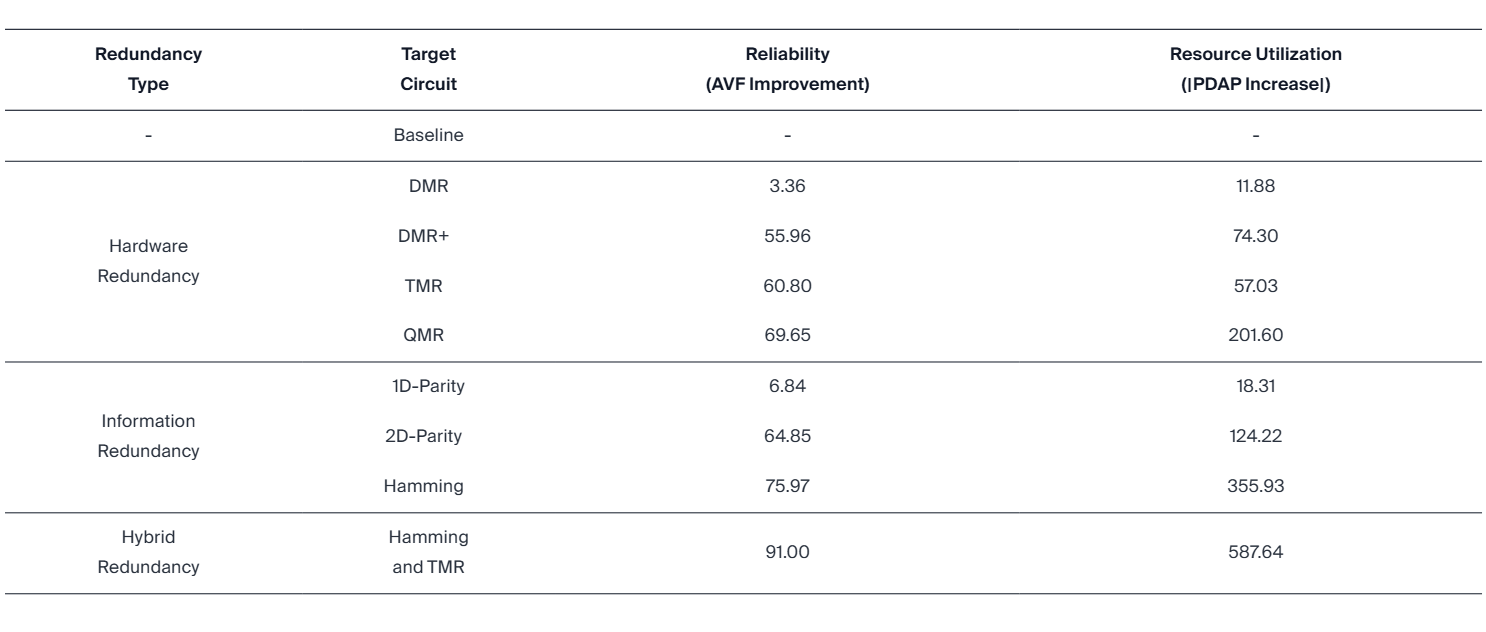
\includegraphics[width=0.9\linewidth] {assets/PDAP.png}
    \caption{Reliability and resource utilization analysis per target circuit}
    \label{fig:PDAP}
\end{figure}

This case study demonstrates that RTL simulation bridges the gap between high-level functional verification and physical implementation. It allows engineers to optimize the "Reliability vs. Resource" cost function before committing to silicon, a capability that neither pure software injection (SWIFI) nor physical emulation can easily provide.